%source mathadata
Un drone survole une zone et se trouve en $D(3\,;\,2)$. Il doit rejoindre une station de recharge avant de tomber en panne de batterie : la station A est en $A(1\,;\,3{,}5)$ et la station B est en $B(5{,}5\,;\,4)$.

	\begin{MADenumerate}
		\begin{multicols}{2}

			\item Placer les points $D$, $A$ et $B$ dans le repère.

			\item Ajouter un point $H$ de même abscisse que $A$ tel que le triangle $AHD$ soit rectangle en $H$. Compléter le tableau :

			\begin{center}
				{
					\setlength{\tabcolsep}{12pt}
					\begin{tabular}{|c|c|c|}
						\hline
						    & $x$ & $y$     \\
						\hline
						$A$ & $1$ & $3{,}5$ \\
						\hline
						$H$ &     &         \\[0.3em]
						\hline
						$D$ & $3$ & $2$     \\
						\hline
					\end{tabular}
				}
			\end{center}

			\item \begin{enumerate}
				\item Calculer $x_D - x_A$. Que représente ce nombre pour le triangle $AHD$ ?
				\item Calculer $y_D - y_A$. Ce nombre peut-il être une longueur ?
				\item Lire la distance $AH$ sur le graphique. Vérifier que $(y_D - y_A)^2 = AH^2$.
			\end{enumerate}

			\item En appliquant le théorème de Pythagore, calculer la distance $AD$.

			\item Calculer de même la distance $BD$.

			\item Quelle station de recharge est à la plus petite distance du drone ?

			\item En s'appuyant sur les questions précédentes, proposer dans l'encadré une formule générale de $AD^2$. Vérifier ensuite la formule avec les valeurs numériques de l'exercice.

			\item (Défi) Si le drone est en $D(10\,;\,12)$, quelle station doit-il choisir ?

			\columnbreak

			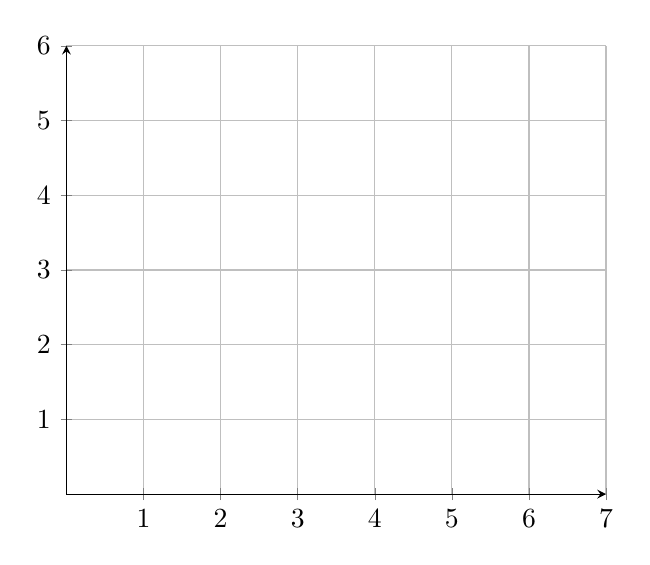
\begin{tikzpicture}
				\begin{axis}[
						xmin=0, xmax=7, ymin=0, ymax=6,
						grid=major,
						axis lines=middle,
						xtick distance=1, ytick distance=1,
						clip=false
					]
					%\addplot+[only marks, mark=*, mark size=2pt] coordinates {(3,2)};
					%\node[anchor=north west] at (axis cs:3,2) {$L$};
				\end{axis}
			\end{tikzpicture}

			\begin{bilan}[Distance entre deux points]
				Soient $A(x_A\,;\,y_A)$ et $D(x_D\,;\,y_D)$ deux points quelconques. Le carré de la distance de $A$ à $D$ est égal à
				$$AD^2 = \ligne[4cm]$$
			\end{bilan}
		\end{multicols}

	\end{MADenumerate}
